\begin{multicols*}{2}
  \begin{headline}[enhanced, tikz={rotate=0}]{Fotios Ptochos Promoted to Professor!}
    \begin{multicols}{2}
    Congratulations to Fotios Ptochos for his promotion to the rank of
    Full Professor, effective November 2022. This promotion recognizes
    Prof. Ptochos' achievements in scholarship, teaching in physics and research in
    high-energy physics (HEP), and his overall service to the CDF and CMS
    Collaborations. He is a Harvard University PhD in physics
    graduate (1998) and has been active in HEP-research, both in detector
    development and physics analyses since 1987. In particular, from 1987
    to 1988 he worked in the development of a technique to monitor the
    purity of Liquid Argon (LAr) for the first ever prototype of the
    ICARUS detector, a technique that was subsequently used in the
    experiment. From 1989 to 1994 he worked in the characterization of
    various Tetramethyl liquids as part of a research project to find
    appropriate warm liquids media for the envisioned calorimeter
    detectors at SSC. He also worked in the construction, installation and
    calibration of the Central Muon Extension (CMX) system for the CDF
    detector. From 1994 to 1996 he developed an algorithm to improve
    electron identification for the CDF end-plug ECAL based on the
    information from the calorimeter and hits on the silicon tracker
    detector. The algorithm led to the development and implementation of
    the PHOENIX tracker system in the CDF-II detector. 
    
    In the period of 2000–2003, he was the coordinator of the group
    responsible for the development, installation, maintenance and
    performance monitoring of the CDF-II Hadronic Calorimeter (HCAL)
    timing system. For the entire period of the Tevatron Run-II
    (2001-2011) he served as the coordinator of the CDF central HCAL
    calibration (CHA and WHA), maintenance and performance group. Since
    2004, when he joined the faculty of the UCY Physics Department, he has
    been involved in the UCY HEP group activities related to the
    construction and running of the CMS ECAL at CERN. In 2009, he
    initiated the involvement of the group in the activities related to
    the CMS tracking detector. He was also involved in the development of
    the dual-readout calorimetry concept in a total absorption HCAL for
    future linear-collider experiments. 
    \columnbreak

    Professor Ptochos has led numerous physics analyses, spanning
    from precision measurements on properties of heavy flavour quark
    production and their use as probes for searching for the SM and SUSY
    Higgs bosons, to searches for BSM physics including SUSY, extra
    dimensions and other exotic processes. He has tremendous experience in
    heavy flavour tagging techniques and algorithms, tau-lepton
    identification techniques and new physics model building. 
    He was the first ever recipient of the \say{Fermi National
      Accelerator Laboratory Fellowship} and has co-coordinated multiple research program
    funded primarily by the European Commission (EC) via \textsc{Marie
    Skłodowska-Curie Actions},  the Cyprus Research Promotion
    Foundation (RPF) through \textsc{Didaktor} or \textsc{Excellence
      Hubs} programs, the European Regional Development Fund, and
    UCY. Professor Ptochos is the author and co-author of more than 
    1700 publications in refereed scientific journals and a member of the
    editorial group in charge for producing the education material
    for the entire Cyprus Secondary Education. In addition, he has
    been the supervisor of the research activities of six postdoctoral
    fellows, five PhD and eleven MSc students, as well as the theses
    projects of more than 20 undergraduate students. 

  % ========================
    \begin{figure}
      \begin{center}
        \leavevmode
        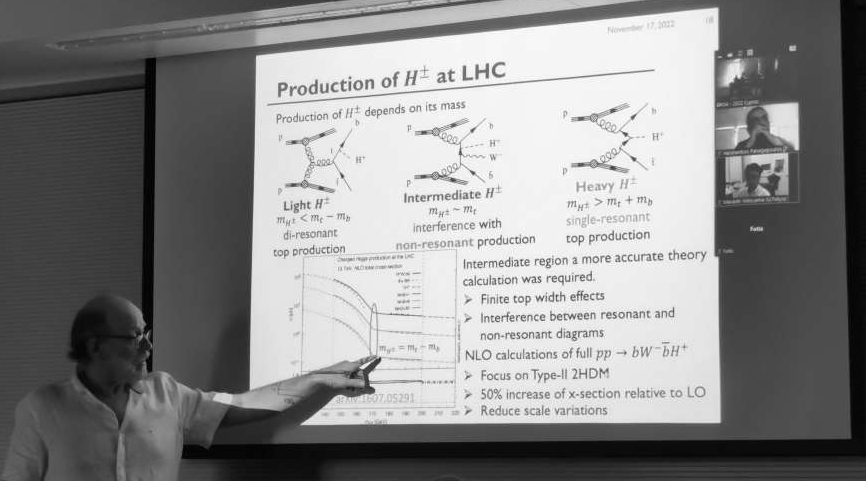
\includegraphics[width=0.5\textwidth]{./figures/Fotis7.png}
      \end{center}
    \end{figure}
    % ========================
    \end{multicols}
  \end{headline}

  \columnbreak
  %\begin{MyArticle}[enhanced, height=0.2\textheight,
%tikz={rotate=0}]{Physicists Find Elusive Particle Seen as Key to
%Universe}
\begin{MyArticle}[enhanced, tikz={rotate=0}, width=0.35\textwidth]{Physicists Find Elusive Particle Seen as Key to Universe}
  \begin{multicols}{2}
    Results are presented from searches for the standard model Higgs
    boson in proton–proton collisions at and 8 TeV in the Compact Muon
    Solenoid experiment at the LHC, using data samples corresponding
    to integrated luminosities of up to 5.1 fb$^{−1}$ at 7 TeV and 5.3 fb$^{−1}$
    at 8 TeV. The search is performed in five decay modes:
    $\gamma\gamma$, $ZZ$,  $\tau^{+}\tau^{-}$, and $b\bar{b}$.
    An excess of events is observed above the expected background,
    with a local significance of 5.0 standard deviations, at a mass
    near 125 GeV, signalling the production of a new particle. The
    expected significance for a standard model Higgs boson of that
    mass is 5.8 standard deviations. The excess is most significant in
    the two decay modes with the best mass resolution, $\gamma\gamma$ and $ZZ$; a
    fit to these signals gives a mass of 
    $125.3\pm0.4(\text{stat.})\pm0.5(\text{syst.}$ GeV. The decay to
    two photons indicates that the new particle is a boson with spin 
    different from one. 
    % ========================
    \begin{figure}
      \begin{center}
        \vspace{-0.2in}
        \leavevmode
        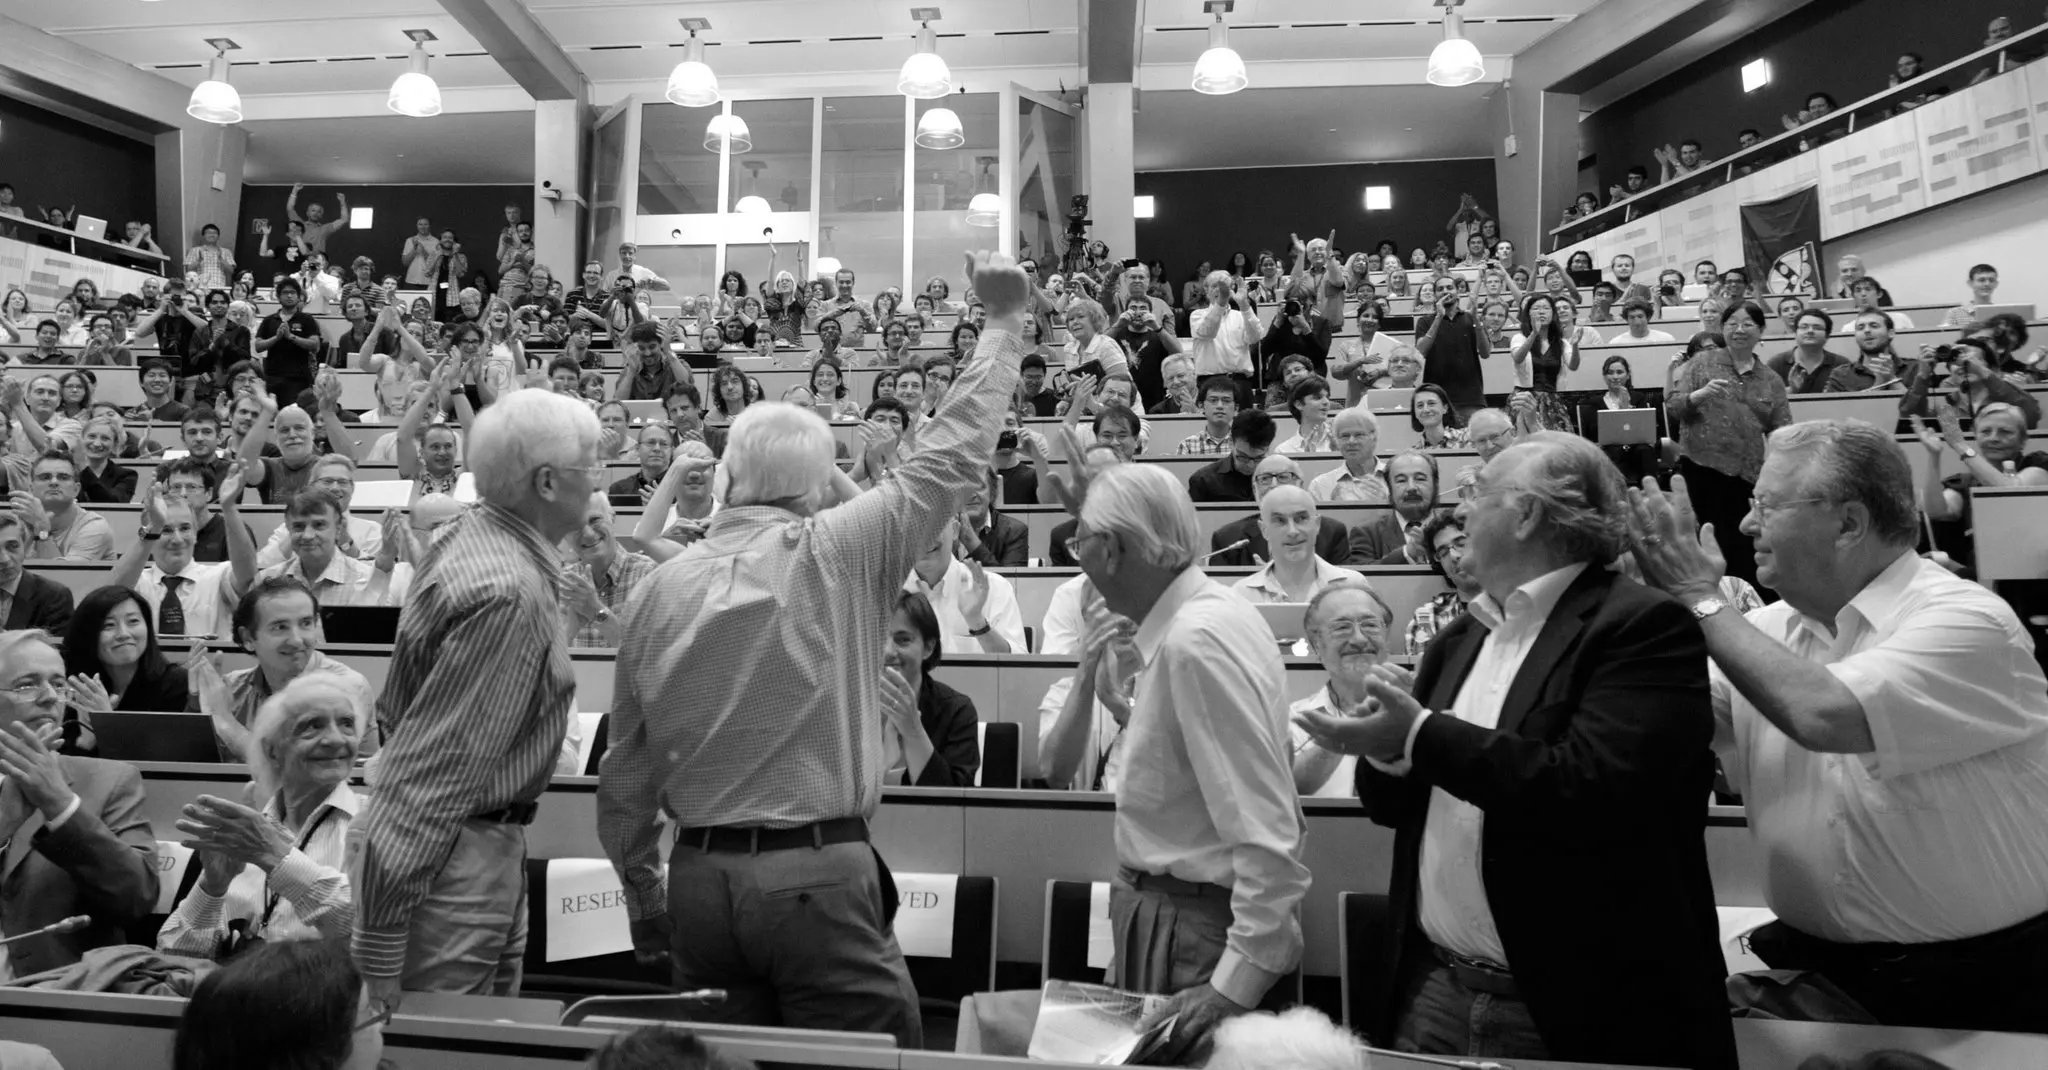
\includegraphics[width=0.5\textwidth]{./figures/HiggsBosonDiscoveryBW.png}
      \end{center}
    \end{figure}
    % ========================
  \end{multicols}
\end{MyArticle}

  %\vfill
  % Ημερίδα πρακτικής άσκησης με δεδομένα από το CERN - Σάββατο 7 Μάρτη 9:00 - 17:00
\begin{MyArticle}[enhanced, tikz={rotate=0}]{Master of Masterclasses \ldots}
  \begin{multicols}{2}
    Another particle physics 
    masterclass was organized at the University of Cyprus by the
    Department of Physics. Thisyear the interest in this event was
    unique and particularlyencouraging. The day \say{Practical Experience with data analysis from
    CERN} was organized by Professor Fotios Ptochos for the 8$^{th}$ year
    in a row and took place within the framework of the
    International Particle Physics Outreach Group (IPPOG)
    effort with the aim of informing the general
    public and especially you students about the research that is
    carried out not only in CERN but also in the wider field of
    Particle Physics. The event you took place on Saturday 07 March
    2020 at the University of Cyprus Campus between 9:00 - 17:00. It 
    included lectures about the world of elementary particles,
    detection methods, and the technology developed starting with basic research in both this and
    related fields of physics. Students had a unique opportunity to
    analyze data from proton-proton collisions, as recorded by the CMS
    detector at CERN's Large Hadron Collider (LHC). They discussed their
    findings with students from other countries as well as scientists
    at CERN through a video conference, during which they also had the
    opportunity to address questions to CERN scientists. 
    % No prior knowledge of particle physics is required, but you may find
    % it easier to read some things before the workshop so you can ask more
    % questions. I am giving you some links below where you can find a lot
    % of information either in English or in Greek:
    % ========================
    \begin{figure}
      \begin{center}
        \leavevmode
        \includegraphics[width=0.5\textwidth]{./figures/Fotis6.png}
      \end{center}
    \end{figure}
    % ========================
  \end{multicols}
\end{MyArticle}

  %\vfill
  %\begin{MyArticle}[enhanced, tikz={rotate=0}]{Top Quark, Last Piece of Matter, Appears to Be in Place}
  \begin{multicols}{2}
    We establish the existence of the top quark using a 67 pb$^{-1}$ data
    sample of pp collisions at $\sqrt{s} = 1.8$ TeV collected with the Collider
    Detector at Fermilab (CDF). Employing techniques similar to those we
    previously published, we observe a signal consistent with $t\bar{t}$ decay to
    $WWbb$, but inconsistent with the background prediction by
    4.8$\sigma$. Additional evidence for the top quark is provided by a peak in
    the reconstructed mass distribution. We measure the top quark mass
    to be $176 \pm 8 (\text{stat.}) \pm 10 (\text{sys.})$ GeV/c$^{2}$,
    and the $t\bar{t}$ production cross section to be
    $6.8^{+3.6}_{-2.4}$ pb.
    % ========================
    \begin{figure}
      \begin{center}
        \vspace{-0.2in}
        \leavevmode
        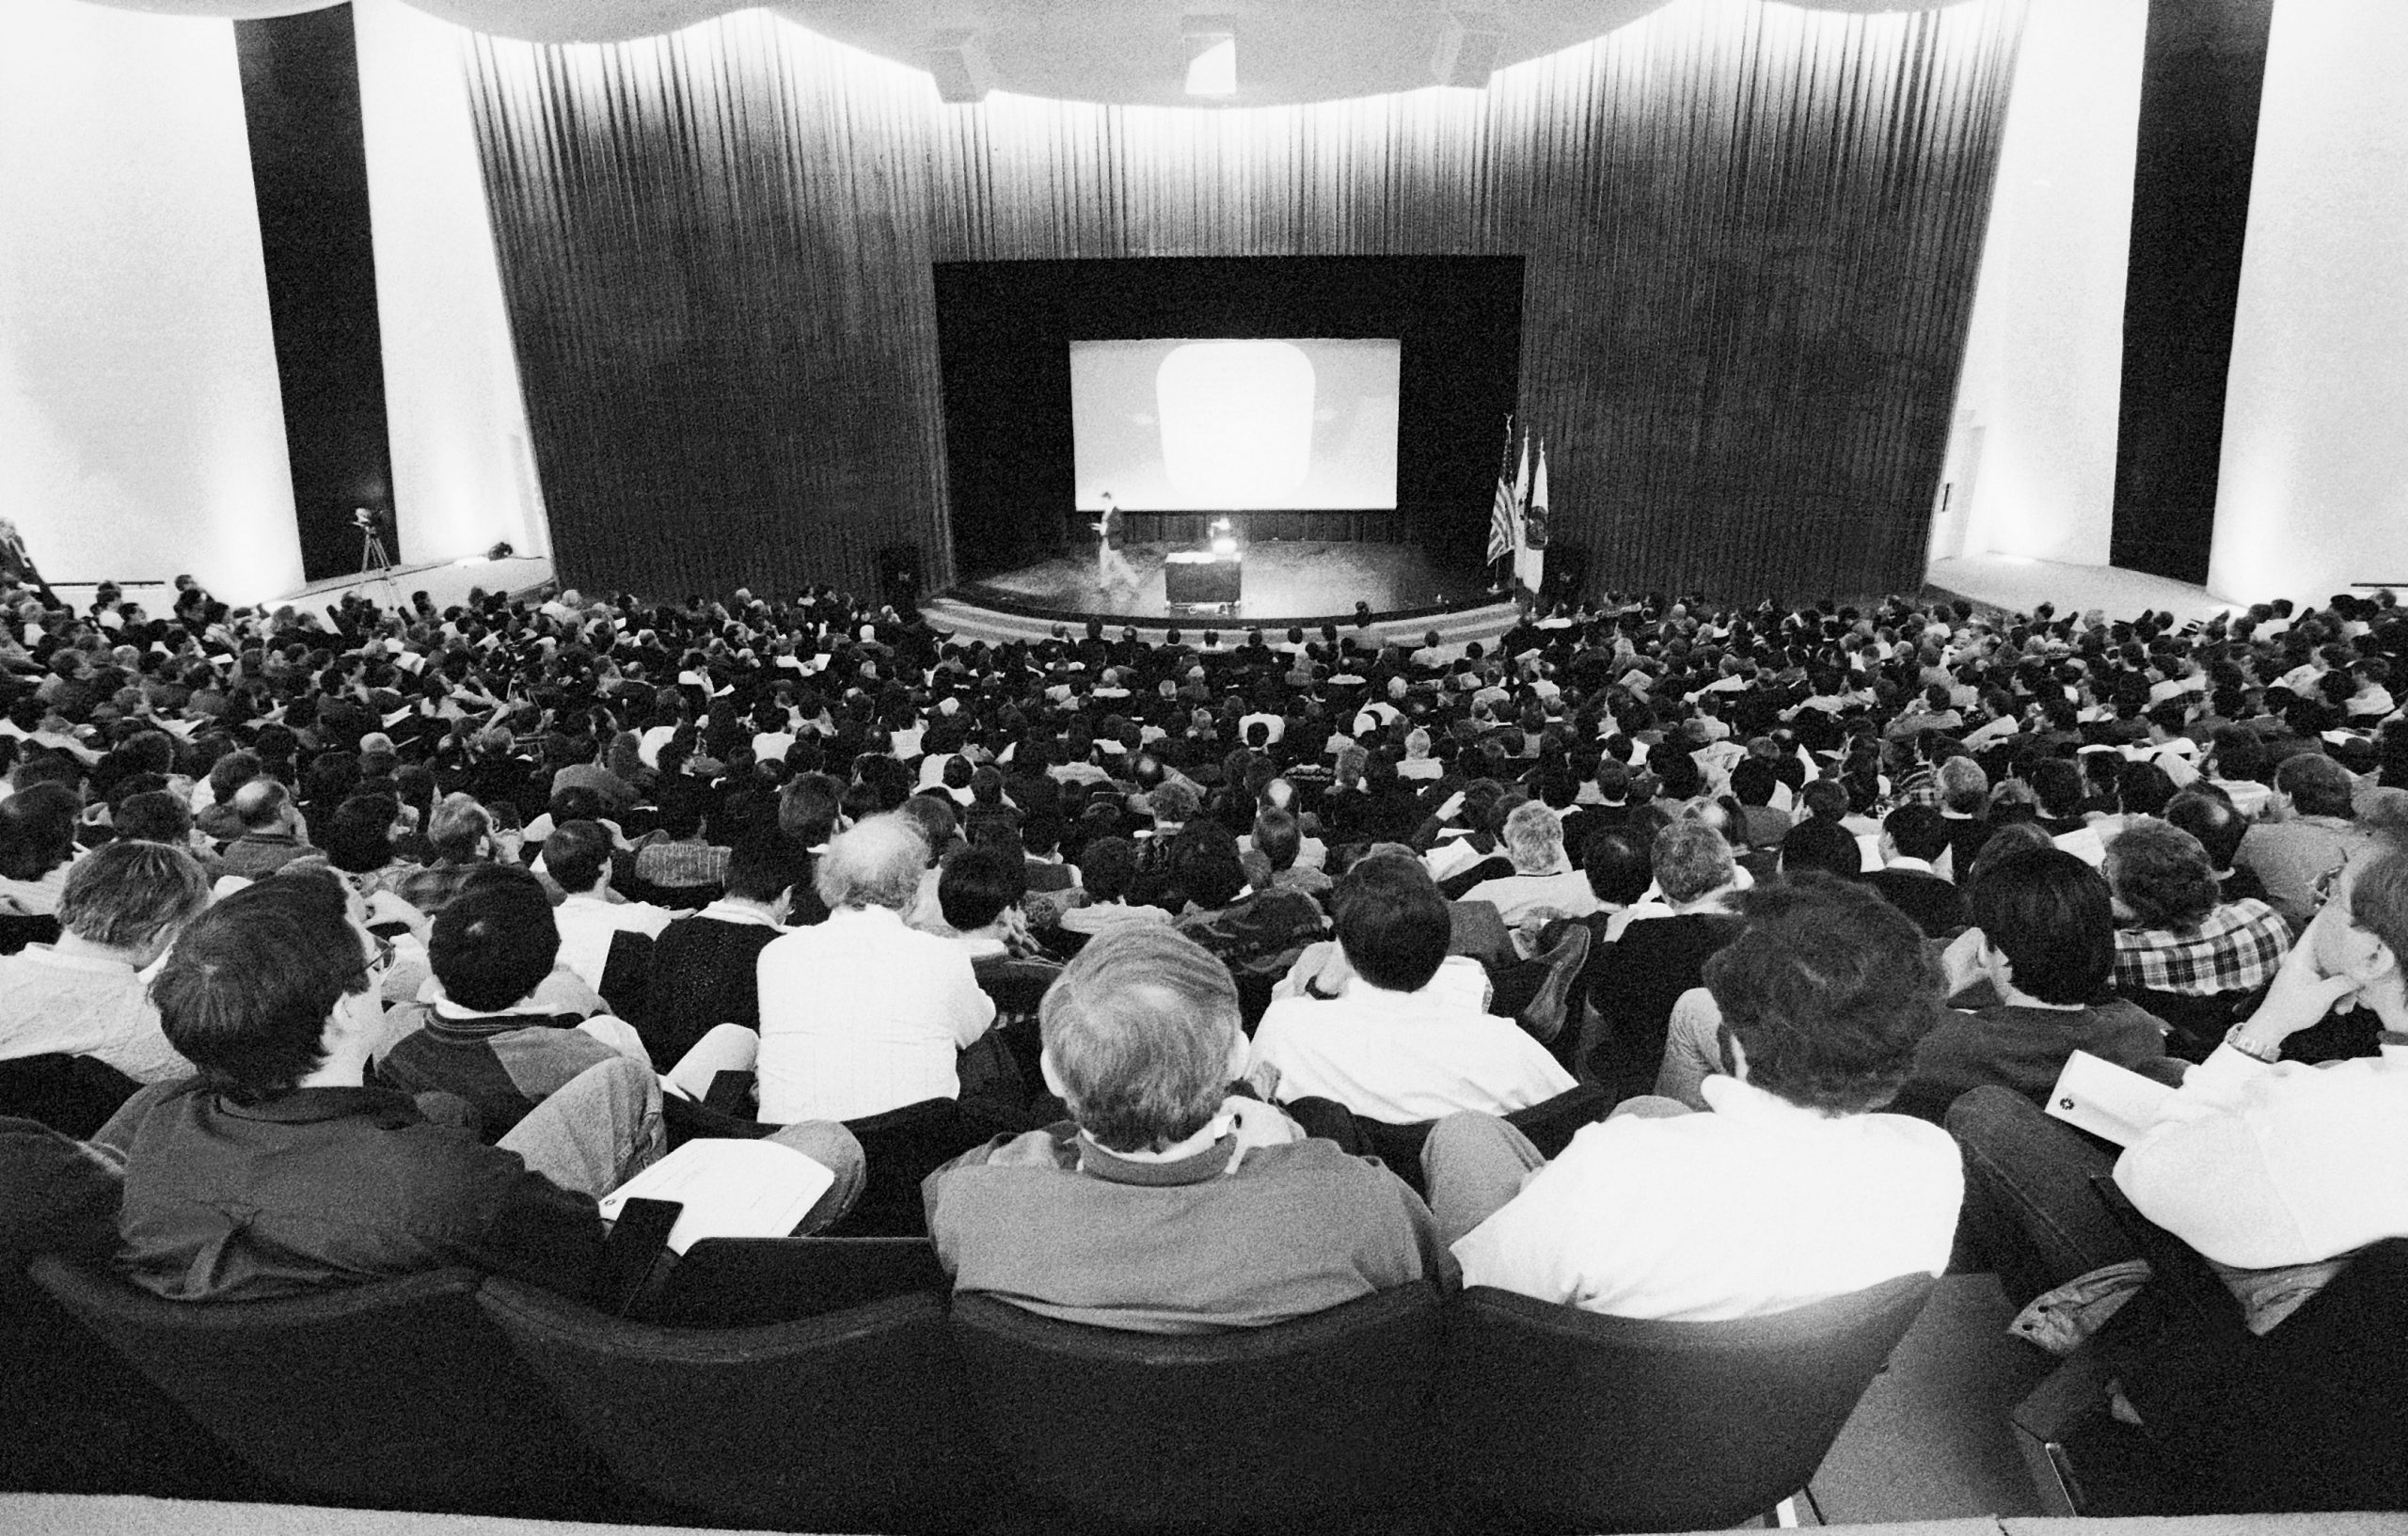
\includegraphics[width=0.5\textwidth]{./figures/TopQuarkAnnouncement.jpg}
      \end{center}
    \end{figure}
    % ========================
  \end{multicols}
\end{MyArticle}

  
\end{multicols*}
